\thispagestyle{empty}
\chapter{Metazoan genome structure and expression}
\vspace*{-10pt}
{\hypersetup{linkcolor=GREYDARK}\minitoc}
\label{chap:intro-metazoan_genome}

My thesis work is focused on the metazoans, commonly known as animals, consisting of arthropods and other clades such as sponges, mollusks, vertebrates, which include fishes, birds, mammals and reptiles. This group appeared around 543-510 million years ago during the cambrian explosion, based on fossil datation~\citep{tikhonenkov_insights_2020}.
Initially, they were characterized based on their morphology. Their primary attributes include being eukaryotes, which implies that their cells possess a complex structure with distinct organelles and a compartmentalized nucleus containing the genetic material. In contrast, prokaryotic species have their genetic material dispersed within the cell's cytoplasm. Another key feature of metazoans is their multicellular nature, wherein an individual consists of multiple cells capable of forming various tissues, and acquiring nutrients by consuming organic matter from other organisms (heterotrophy).

Because metazoans present a wide variety of genomes architecture and biological traits, they provide an exciting opportunity to explore the interplay between genomes evolution and the biology of organisms. Moreover, many data are available for this group of species. 

This section aims to explore the fundamental aspects of metazoans' genome structure and the mechanisms that determine its expression. The objective is to gain a comprehensive understanding of the genomic components investigated in my study.


\section{Genomes content}

The genome, which can be subdivided into one or more fragments called chromosomes, contains the individual genetic material and is inherited by future generations through reproduction. In metazoans, as in most/all living beings, the genome consists of double-stranded molecules of deoxyribonucleic acid (\acrshort{DNA}), this structure was untangled by several scientists in 1953~\citep{franklin_molecular_1953, watson_molecular_1953, wilkins_molecular_1953}. The genetic information is composed of four nucleotides: pyrimidine bases cytosine (\acrshort{C}), thymine (\acrshort{T}), and purine bases adenine (\acrshort{A}), guanine (\acrshort{G}). These nucleotides \acrshort{A}, \acrshort{G}, \acrshort{C}, and \acrshort{T} are present in \acrshort{DNA}, with \acrshort{T} bonding to \acrshort{A} and \acrshort{G} bonding to \acrshort{C} through hydrogen bonds. The directionality of a single strand of \acrshort{DNA}, called 5' and 3' ends, is determined by the position of chemical elements (\hyperref[fig:dnamolecule]{Fig. 1.1}). This orientation and the sequence of nucleotides determine the genetic information encoded in the genome.

\begin{figure}[ht]
    \centering
    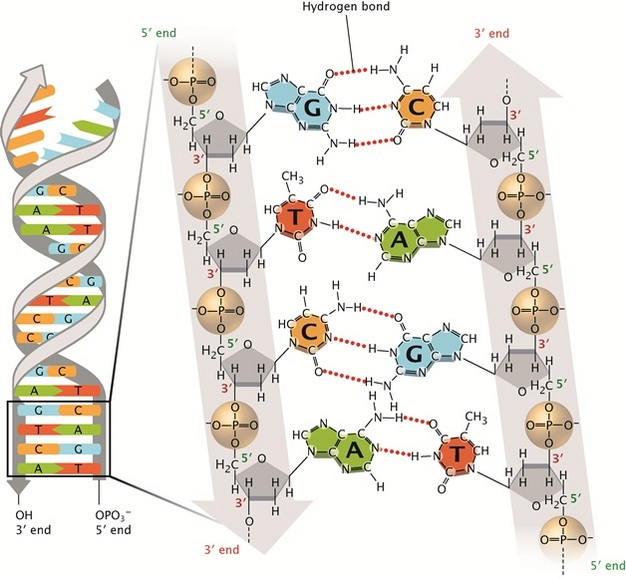
\includegraphics[width=0.8\linewidth]{figures/dna_molecule.jpg}
    \caption[DNA molecule]{\textbf{DNA molecule.} Double-stranded molecules of deoxyribonucleic acid (DNA), illustrating the structural and atomic bonds connecting each nucleobase. \\
    \scriptsize{Reproduced from Springer Nature for a noncommercial use.}}
    \label{fig:dnamolecule}
\end{figure}
% (confirmation email from Jean Davis of the Online Service Specialist received on December 8th , 2023
    % \url{https://www.nature.com/scitable/topicpage/discovery-of-dna-structure-and-function-watson-397/}

The size of the haploïd genome in metazoans varies significantly, ours is 3.2 \acrshort{Gb} (104 cm,~\citet{piovesan_length_2019}). On average, metazoan genomes tend to be around 1 \acrshort{Gb} in size~\citep{hotaling_toward_2021}. Remarkably, the \textit{Australian lungfish} boasts a genome 14 times larger than that of humans, measuring approximately 43 \acrshort{Gb}~\citep{meyer_giant_2021}. On the other hand, the marine parasite \textit{Intoshia variabili} possesses the smallest known animal genome, measuring only 15.3 \acrshort{Mb}~\citep{slyusarev_extreme_2020}. Nevertheless, it is essential to acknowledge that not all genomes have been measured to date, leaving room for further discoveries and variations in genome sizes across the animal kingdom.

The genome comprises distinct regions with diverse functions, including coding regions that oversee protein synthesis and non-coding regions. Remarkably, a significant proportion of our genome, approximately 98.5\%, is comprised of non-coding regions. In stark contrast, only a mere 1.5\% of the genome encompasses coding regions responsible for protein synthesis. These coding regions are found within protein-coding genes making up nearly one-third of the entire genome~\citep{lander_initial_2001, venter_sequence_2001, international_human_genome_sequencing_consortium_finishing_2004}.



\section{Genes: holder of genetic information}
\label{sec:genes}

The concept of `gene' has undergone changes in its definition since its first mention as `inherited cell elements' by~\citet{mendel_versuche_1866}. The word `gene' was subsequently introduced by~\citet{johannsen_elemente_1909} and quickly became essential in the emerging field of genetics. Nowadays, a definition of a gene in eukaryotic organisms could be: `a transcription unit, whose expression leads to the production of a functional molecule (\acrshort{RNA} or protein)'. Transcription being the first step of gene expression (see `\nameref{sec:transcription}' section). Genes can be broadly classified into two main categories: the first category includes non-coding \acrshort{RNA}, such as transfer \acrshort{RNA}s (\acrshort{tRNA}s), ribosomal RNAs (rRNAs), microRNA (21-25 nucleotides) responsible for controlling expression~\citep{filipowicz_mechanisms_2008, obrien_overview_2018} and long \acrshort{RNA} molecules (greater than 200 nucleotides) known as \acrshort{lncRNA}~\citep{kashi_discovery_2016}.

The second category comprises protein-coding genes that encode proteins. Protein-coding genes exhibit substantial variation in size across different species. For instance, in humans, the median gene size is approximately 24 \acrshort{kb} \citep{fuchs_4sudrb-seq_2014}, whereas in diptera \textit{Drosophila melanogaster}, genes are comparatively shorter with a median size of 2 \acrshort{kb} for its 14,000 protein-coding genes (assembly GCF\_000001215.4). Additionally, there are pseudogenes, which are remnants of protein-coding genes that have either lost their function over time or are not transcribed. In humans, there are 8,700 pseudogenes annotated (assembly GCF\_000001405.38,~\citet{mighell_vertebrate_2000}).

Protein-coding genes in metazoans follow a specific structure. Upstream of a gene is a promoter sequence that plays a crucial role in activating the first step of gene expression, its transcription (\hyperref[fig:genestructure]{Fig. 1.2}). This region is responsible for attracting \acrshort{RNA} polymerase II, the enzyme responsible for initiating its expression.

\begin{figure}[ht]
    \centering
    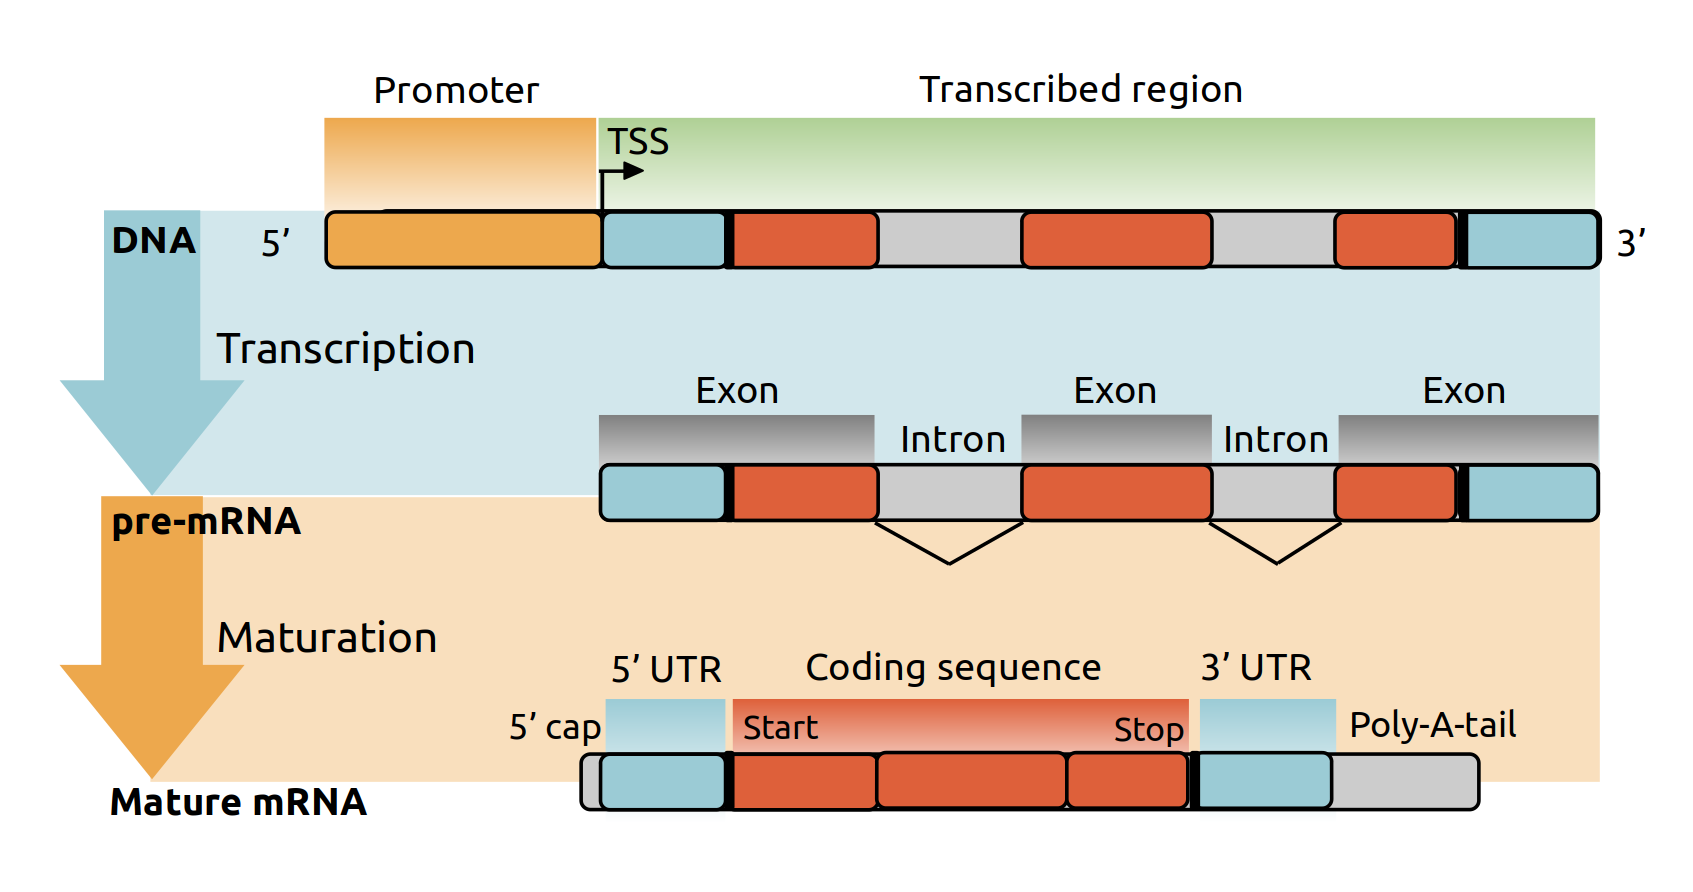
\includegraphics[width=\linewidth]{figures/gene_structure.png}
    \caption[Gene structure and expression]{\textbf{Gene structure and expression.} Schematic representation of an eukaryotic gene and its structural components, including the promoter, transcription start site (\acrshort{TSS}), untranslated transcribed regions (\acrshort{UTR}), coding sequence (\acrshort{CDS}), as well as introns and exons. A concise overview of key processes such as transcription of DNA and maturation of pre-\acrshort{mRNA} is provided to appreciate the mechanisms underlying gene expression.\newline}
    \label{fig:genestructure}
\end{figure}

Following the promoter there is the transcribed region of a gene. This region consist of alternating sequences known as exons and introns. Exons constitute the protein coding region (\acrshort{CDS}) and its 5' and 3' untranslated regions, whereas introns are non-coding sequences and represent 25\% of our genome~\citep{sakharkar_distributions_2004}. A recent investigation encompassing 1,700 species reveals that the primary origin of continuous intron formation in eukaryotic genomes stemmed from introners, which are transposable elements capable of creating copies of themself that insert into many genes throughout the genome, akin to intragenomic parasitic elements~\citep{gozashti_transposable_2022}. Not all genes contain introns, we called multiexonic genes those with both exons and introns. The fraction of multiexonic genes is high but varies slightly between species, \textit{e.g.} 90\% in fly and 95\% in \textit{Homo sapiens}. In human, the coding regions of multiexonic genes typically contains an average of 8 introns with a median length of 1,747 \acrshort{bp}, and 9 exons with a median length of 131 \acrshort{bp}~\citep{piovesan_human_2019}. These characteristics vary widely between species, in number: 4 exons per gene in dipterans to 10 exons in vertebrates, and in length: on average, the introns measure 1,000 \acrshort{bp} in vertebrates, 1,200 \acrshort{bp} in mammals, 850 \acrshort{bp} in birds to 80 \acrshort{bp} in dipterans.

In the final product of transcription, the coding sequence is flanked by Untranslated Transcribed Regions (\acrshort{UTR}s). The 5' \acrshort{UTR} region serves as the site where the ribosome enzyme attaches to initiate translation. On the other hand, the 3' \acrshort{UTR} region plays a role in translation termination, \acrshort{mRNA} stability and localization (\citet{ grzybowska_regulatory_2001, chabanon_zipcodes_2004, mayr_what_2019}; see `\nameref{sec:translationdecoding}' section).

Many protein-coding genes have been identified: less than 6,000 in yeast, 14,000 in \textit{Drosophila melanogaster}, 26,000 in \textit{Arabidopsis thaliana}. Initially, prior to the sequencing of the human genome, estimates suggested that up to 140,000 genes could be present~\citep{fields_how_1994}. Indeed it was expected, due to assumptions and anthropocentric perspectives, that the human being the most complex species of all, would possess a large number of genes. However, the first large-scale comparative analysis of vertebrate genomes revealed a modest count of $\approx30,000$ genes in our genome \citep{roest_crollius_estimate_2000}, later confirmed by the Genome Sequencing Consortium \citep{lander_initial_2001, venter_sequence_2001}. Following improvement in the assembly and annotation, the current estimation dropped to around 20,000 genes~\citep{clamp_distinguishing_2007, ezkurdia_multiple_2014, piovesan_human_2019}. While the notion of organism complexity is difficult to define and subject to anthropocentric bias, its discrepancy with gene count, known as the G-value paradox, continues to be the subject of intense investigation and raises numerous questions~\citep{hahn_g-value_2002, straalen_introduction_2011, choi_c-_2020}. 

\section{RNA transcription and maturation process}
\label{sec:transcription}

Protein-coding genes are expressed through the transcriptional process, involving the transcription of DNA into premature \acrshort{RNA} (pre-\acrshort{mRNA}), which subsequently undergoes maturation to yield the mature messenger \acrshort{RNA} (\acrshort{mRNA}).

\subsection{Transcription}

Transcription of protein-coding genes takes place within the nucleus, where \acrshort{RNA} polymerase II synthesizes a ribonucleic acid (\acrshort{RNA}) molecule~\citep{nikolov_rna_1997}. \acrshort{RNA} polymerase II's attachment is facilitated by the recognition of specific elements such as the TATA box and/or initiator (Inr;~\citet{emami_mechanism_1997}). The TATA box is typically positioned approximately 25 \acrshort{bp} upstream of the transcription start site (TSS; \hyperref[fig:genestructure]{Fig. 1.2};~\citet{lifton_organization_1978}).

During elongation, the \acrshort{RNA} polymerase moves in a 5' to 3' direction, transcribing the DNA into a single-stranded RNA molecule. In this RNA molecule, thymine (\acrshort{T}) is replaced by uracil (\acrshort{U}), while the other nucleotides remain unchanged. The primary distinction between deoxyribonucleic acid (DNA) and ribonucleic acid (RNA) lies in the presence of a hydroxyl group (OH) which is a reason for the relative instability of \acrshort{RNA} compared to DNA \citep{ross_mRNA_1995, wang_origins_1995, fordyce_long-term_2013}. 

Termination of transcription occurs when \acrshort{RNA} polymerase II reaches a terminator region signal \citep{birse_transcriptional_1997, proudfoot_transcriptional_2016}. At this point, transcription is completed, and the \acrshort{RNA} molecule dissociates from the \acrshort{DNA}. This \acrshort{RNA} molecule is referred to as premature RNA.


\subsection{Maturation}

Premature \acrshort{RNA} undergoes three distinct pre-processing steps during transcription in the nucleus. The first step involves the addition of a 7-methylguanosine at the 5' end of the pre-\acrshort{mRNA} by a guanylyltransferase, called 5'-cap (\hyperref[fig:genestructure]{Fig. 1.2}). Subsequently, this 7mG (7-methylguanosine) cap structure is recognized by the cap binding complex (CBC; \citet{gonatopoulos-pournatzis_cap-binding_2014}). 
The cap structure bound to CBC is believed to play a crucial role in \acrshort{mRNA} stabilization~\citep{beelman_degradation_1995}.
Additionally, in the cytoplasm, the cap bound to translation initiation factors to promote translation by facilitating the interaction between the \acrshort{mRNA} and ribosomal subunits (see \nameref{sec:translationdecoding}).

The second maturation step is splicing. In 1977, research by the Sharp and Roberts labs, as well as Chambon lab, revealed that genes are composed of multiple distinct segments along the DNA molecule~\citep{berget_spliced_1977, breathnach_ovalbumin_1977, breathnach_organization_1981, berk_discovery_2016, suran_finding_2020}. Indeed, in eukaryotes, most genes are interrupted by introns, which are removed from the pre-\acrshort{mRNA}. 

Splicing occurs through two transesterification reactions: first, the hydroxyl group of the donor site reacts with the branch point adenosine nucleotide, and then the donor site reacts with the acceptor site, resulting in the excision of the intron and exon–exon ligation. The resulting intron structure forms a `lariat structure'~\citep{proudfoot_integrating_2002}.

This process is carried out by a macromolecular complex, the spliceosome, which includes five small nuclear RNAs (snRNAs) known as U1, U2, U4, U5, and U6, as well as approximately 200 proteins~\citep{lerner_are_1980, mount_recognizing_2015}. This spliceosome recognizes specific exon/intron boundaries, 5' and 3' splice sites, the donor site marked by the dinucleotide GU (but also GC;~\citet{aebi_5_1987}), and the acceptor site marked by the dinucleotide AG~\citep{breathnach_ovalbumin_1978}. A minor subclass of introns was further discovered, with AU-AC boundaries, excised by a second spliceosome composed of U11, U12, U4atac, U6atac and U5 snRNAs. Based on the spliceosome pathway that takes in charge their removal, introns are categorized U2-type or U12-type~\citep{sharp_classification_1997}

In the last phase of transcription maturation a specific sequence of nucleotides known as a poly(A) tail (\hyperref[fig:genestructure]{Fig. 1.2}) is appended to the 3' end of the transcribed RNA molecule at the polyadenylation signal (PAS). This tail consists of approximately 250 adenine nucleotides in mammalian cells and is synthesized by an enzyme called poly(A) polymerase~\citep{xiang_molecular_2021}. The addition of this poly(A) tail plays a crucial role in enhancing the stability of the RNA molecule by enabling its interaction with the poly(A)-binding protein, thereby protecting it from enzymatic degradation~\citep{preiss_end_2013, nicholson_tales_2019, passmore_roles_2022}. 

Consequently, the resulting RNA molecule is called mature \acrshort{mRNA}. Once fully developed, mature \acrshort{mRNA} molecules are transported out of the nucleus to undergo translation. mRNA are much less stable than DNA and eventually degrade, which can serve to modulate gene expression over time after gene transcription \citep{ross_mRNA_1995, wang_origins_1995, fordyce_long-term_2013}. 

\section{Alternative splicing}

In addition to the discovery of RNA splicing, another yet surprising observation was that not only pre-\acrshort{mRNA} contains introns that needed to be excised, but also alternative patterns of splicing could lead to different mature messenger \acrshort{RNA}s from a same pre-\acrshort{mRNA} molecule. The first example was observed in adenovirus where one pre-\acrshort{mRNA} molecule could be spliced at different junctions to produce different mature \acrshort{mRNA}s, with different combination of exons, called alternative splicing (\acrshort{AS})~\citep{berget_spliced_1977, berk_discovery_2016}. Three years later alternative splicing was found in immunoglobulin genes of mouse myeloma tumors cells~\citep{early_two_1980}.

Different patterns of alternative splicing have then been described such as exon skipping, where an exon is omitted; intron retention, where an intron is retained; 5' and 3' alternatively spliced site, where different splice sites are selected for splicing; and mutually exclusive exons, where only one of two exons is present (\hyperref[fig:asevents]{Fig. 1.3};~\citet{wang_splicing_2008}).

Soon, the scientific community has tended to draw direct conclusions about the `raison d'être' of alternative splicing. It has been proposed that \acrshort{AS} serves as a mean to enhance the functional diversity of species genomes, thereby providing a straightforward explanation for the G-value paradox previously discussed (see \nameref{sec:genes};~\citet{graveley_alternative_2001}). Indeed, if the number of genes alone cannot account for the complexity of an organism, the expansion of the protein repertoire by alternative splicing could be the missing part of the equation. % Indeed, if the number of genes alone cannot account for the complexity of an organism, it is plausible that accounting for the expansion of protein repertoire by AS is the missing part of the equations. % as it could increase the proteins repertoire. renders the direct correlation between gene count and protein production unreliable. 
Notably, studies have demonstrated that \acrshort{AS} is predominant in humans and primates, which are, by some, considered complex species, where more than 90\% of multiexonic protein coding genes undergo alternative splicing~\citep{wang_alternative_2008, pan_deep_2008}, compared to 35\% in the nematode \textit{Caenorhabditis elegans} and 20\% in the fly \textit{Drosophila melanogaster}~\citep{chen_correcting_2014}.


\begin{figure}[ht]
    \centering
    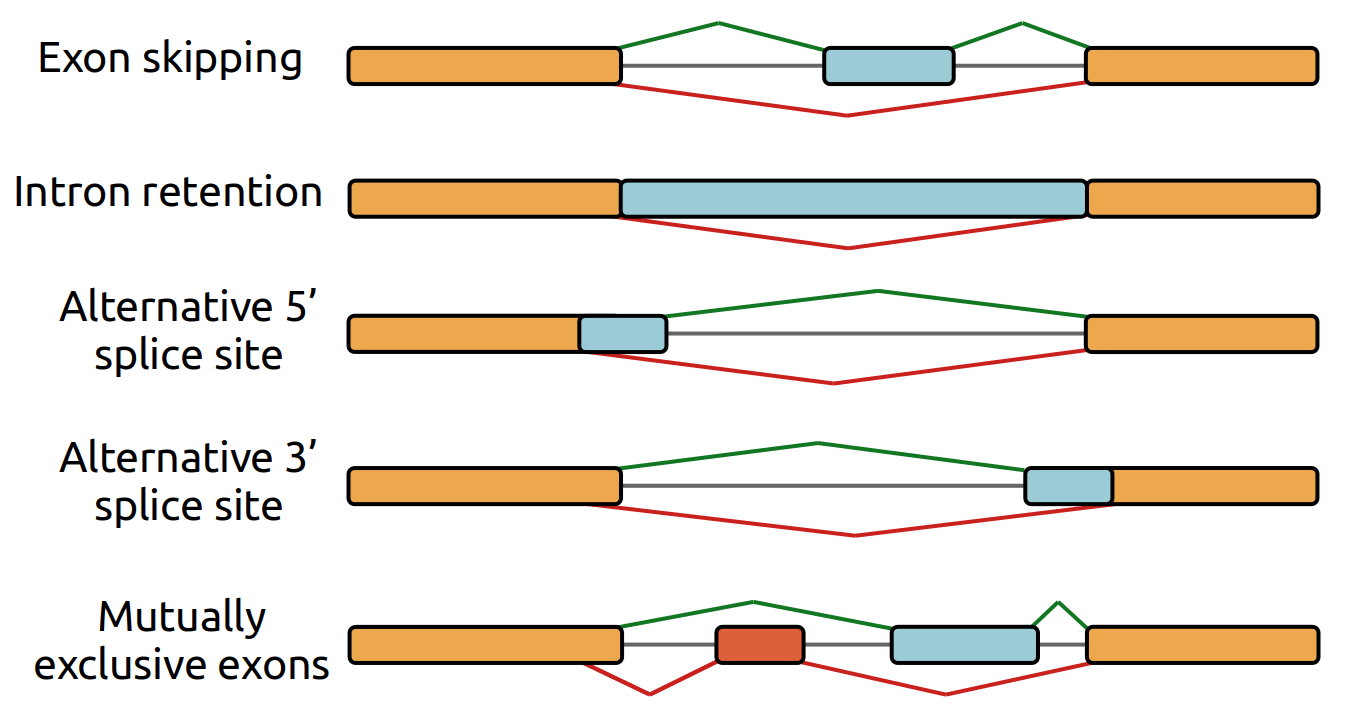
\includegraphics[width=0.7\linewidth]{figures/as_events.png}
    \caption[Alternative splicing events]{\textbf{Alternative splicing events.} Schematic view of the different pattern of alternative splicing such as exon skipping, where an exon is omitted; intron retention, where an intron is retained; 5' and 3' alternatively spliced site, where different splice sites are selected for splicing; and mutually exclusive exons, where only one of two exons is present. Exons are presented using boxes (unless an intron is retained), introns with lines. Orange exons correspond to constitutive ones.\newline}
    \label{fig:asevents}
\end{figure}

Extensive research, observations, and reviews have shown that \acrshort{AS} can undoubtedly lead to the generation of distinct functional proteins from a single gene~\citep{blencowe_alternative_2006, ule_alternative_2019, wright_alternative_2022, verta_role_2022, singh_importance_2022}. Recently, AS has gained significant research focus, particularly in the field of cancer, where its alterations and crucial involvement in tumor proliferation have been extensively investigated~\citep{anczukow_splicing-factor_2016, bonnal_roles_2020, qi_significance_2020}. Thus, \acrshort{AS} has emerged as a promising therapeutic target for novel cancer treatments that aim to disrupt oncogenic splicing events or target upstream splicing regulators~\citep{sciarrillo_role_2020}.

However, it is also important to consider that splicing errors by the splicing machinery can contribute to this variability~\citep{pickrell_noisy_2010, rajon_evolution_2011, xu_alternative_2018, saudemont_fitness_2017}. Indeed, the splicing machinery's precision is not infallible, and like any intricate process, it is susceptible to inaccuracies that can lead to the formation of aberrant transcripts. The extent to which erroneous splicing outpaces functional splicing remains a topic of substantial debate within the scientific community~\citep{tress_alternative_2017, blencowe_relationship_2017, tress_most_2017}, especially given the high occurrence of alternative splicing in humans~\citep{pan_deep_2008}. My research aims to bring new answers to this ongoing debate, and I explore this topic in the subsequent `\nameref{chap:intro-objectives}' section.



\section{Translation and decoding via the genetic code}
\label{sec:translationdecoding}
Once the mature \acrshort{mRNA} molecule is produced, it is exported to the cytoplasm where it is translated into proteins. This spatial decoupling between transcription/maturation/splicing (in the nucleus) and translation (in the cytoplasm) allows the process of splicing to occur prior to the initiation of protein sequence synthesis.

First, the \acrshort{mRNA} is positioned near the endoplasmic reticulum (ER), a cellular structure containing numerous ribosomes~\citep{palade_small_1955}. These ribosomes are responsible for \acrshort{RNA} translation into protein in accordance with the genetic code, which establishes the correspondence between the DNA sequence and the amino acid sequence of a protein~\citep{balis_role_1958}. 

Initially, the eukaryotic ribosome's small subunit (40S) and three initiator factor proteins (IF1, IF2, and IF3) forms a preinitiation complex (PIC) to the 5'-cap of \acrshort{mRNA}s~\citep{wang_rapid_2022}. The PIC scans the \acrshort{UTR} until it finds a ribosome-binding site (RBS;~\citet{kozak_scanning_1989}). On this site an initiation complex is formed with the recruitment of the large ribosome subunit (60S;~\citet{blanchet_translation_2022}). Then, \acrshort{mRNA} sequence is read in triplets of nucleotides known as codons, starting from the initiation codon downstream of the RBS. Each codon corresponds to a transfer RNA (\acrshort{tRNA}) molecule. In eukaryotes, tRNA are 90-nucleotide-long molecules produced by RNA polymerase III, and bound to the proper amino acid by aminoacyl-tRNA synthetase enzymes~\citep{sprinzl_-c-c-end_1979}. tRNAs function by recognizing and binding to the complementary codon through the traditional Watson-Crick base pairing. Additionally, tRNAs undergo post-transcriptional modifications, enabling them to engage in non-Watson-Crick base pairing and unconventional interactions~\citep{percudani_restricted_2001}. Notably, adenosine (\acrshort{A}) can be modified to inosine (\acrshort{I}) through post-transcriptional deamination, allowing for permissive wobble pairing such as I:C, I:U, or I:A (\hyperref[fig:pairing]{Fig. 1.4}). Another common wobble pairing involves G:U/U:G base pairing~\citep{percudani_restricted_2001}.

The initiation of translation begins at the start \gls{codon} `AUG', where a methionine is attached to the tRNA and positioned on the ribosome~\citep{tamura_origins_2015}. As loaded \acrshort{tRNA}s bind, the ribosome progresses along the \acrshort{mRNA}, utilizing three distinct slots: the A-site, P-site, and E-site. The A-site serves as the initial binding site for the \acrshort{tRNA}, the P-site holds the \acrshort{tRNA} connected to the growing polypeptide chain, and the E-site is the exit site.

While each codon corresponds to an amino acid, there are more codons than there are amino acids. This redundancy in the genetic code implies that multiple codons can encode the same amino acid, called \gls{synonymous} codons. To study \gls{codon usage} (\acrshort{CU}) variations between metazoans, \gls{GC-content} (\textit{i.e.} \acrshort{G}+\acrshort{C} fraction) at the third position of the codons (\acrshort{GC3}) is often used because it is the most \gls{synonymous} position of the three positions. It has long been observed that \gls{synonymous} codons usage is uneven across taxa, with a \acrshort{GC3} varying from 20\% in some hymenopterans to 60\% in mammals and up to 70\% in some dipterans. Codon usage also varies within genomes, between genes~\citep{grantham_codon_1980, grantham_codon_1980-1, gouy_codon_1982, ikemura_codon_1985, parvathy_codon_2022}. 

\begin{figure}[ht]
    \centering
    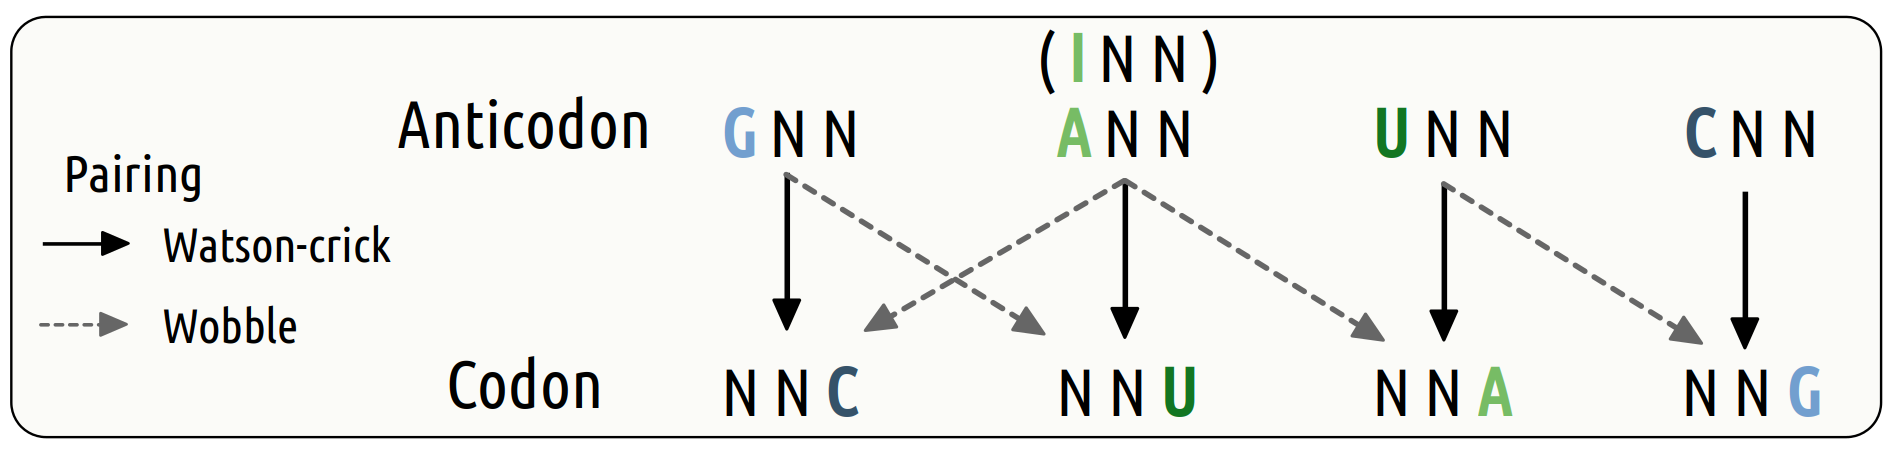
\includegraphics[width=0.8\linewidth]{figures/wobble_pairing.png}
    \caption[Watson-Crick and wobble pairing]{\textbf{Watson-Crick and wobble pairing.} The panel illustrates the various possible pairings: Watson-Crick and wobble pairing (\textit{i.e.} I:C, I:U, I:A and G:U/U:G).\newline}
    \label{fig:pairing}
\end{figure}


Even though modification in the use of \gls{synonymous} codons do not change the encoded protein, several evidences indicate that they influence gene expression~\citep{hershberg_selection_2008, plotkin_synonymous_2011, martinez_synonymous_2019, liu_synonymous_2021}: transcription regulation in \textit{Neurospora}~\citep{zhou_codon_2016, zhao_genome-wide_2021} and in human~\citep{fu_codon_2018}; translation initiation~\citep{eyre-walker_reduced_1993, bhattacharyya_accessibility_2018, goodman_causes_2013} and elongation~\citep{sorensen_codon_1989, boel_codon_2016} in \textit{Escherichia coli}; translation accuracy in \textit{Drosophila melanogaster}~\citep{akashi_synonymous_1994}, in \textit{Escherichia coli}~\citep{stoletzki_synonymous_2007}, in yeast, worm, fly, mouse, human~\citep{drummond_mistranslation-induced_2008} and in bacterial taxa~\citep{sun_preferred_2022}; \acrshort{RNA} stability in \textit{Saccharomyces cerevisiae}~\citep{presnyak_codon_2015}, \textit{Schizosaccharomyces pombe}~\citep{harigaya_analysis_2016}, \textit{Homo sapiens}~\citep{hia_codon_2019} and in \textit{Escherichia coli}~\citep{kudla_coding-sequence_2009}; protein folding~\citep{drummond_mistranslation-induced_2008, buhr_synonymous_2016, walsh_synonymous_2020}; \acrshort{RNA} splicing in mouse, human~\citep{pagani_synonymous_2005} and HIV-1~\citep{takata_global_2018}; \acrshort{RNA} toxicity in \textit{Escherichia coli}~\citep{mittal_codon_2018}.

Previous studies on model organisms such as \textit{Escherichia coli}~\citep{ikemura_correlation_1981}, \textit{Saccharomyces cerevisiae}~\citep{ikemura_codon_1985} and \textit{Caenorhabditis elegans}~\citep{duret_trna_2000} have demonstrated that the most frequently used codons are decoded by the most abundant \acrshort{tRNA} molecules suggesting a co-adaptation between the \acrshort{tRNA} pool and \gls{codon usage}~\citep{ikemura_codon_1985}. Also, in those species, highly expressed genes, which are likely to be under selection for translation optimization, exhibit a preference for codons associated with abundant tRNA molecules, which is interpreted as a selection on codons usage~\citep{ikemura_correlation_1981, percudani_transfer_1997, duret_trna_2000, plotkin_codon_2006, plotkin_synonymous_2011, quax_codon_2015}. Indeed, to optimize translation the utilization of codons that align with the most prevalent \acrshort{tRNA} molecules accelerates the process of locating and attaching ribosome to the appropriate tRNA, thereby diminishing the probability of associating with a non-cognate \acrshort{tRNA}~\citep{dana_effect_2014, quax_codon_2015}.

While selection on \gls{synonymous} codons to optimize translation, called \gls{translational selection} (\acrshort{TS}), has been observed in some model species though rarely in vertebrates~\citep{doherty_translational_2013}, we still lack a comprehensive study that embrace numerous metazoans. Also, in human there is still a debate on whether \acrshort{TS} is modulating the choice of \gls{synonymous} codons~\citep{comeron_selective_2004, semon_no_2006, doherty_translational_2013, gingold_dual_2014, pouyet_recombination_2017, dhindsa_natural_2020}. I will provide a more detailed discussion on \gls{translational selection} in the `\nameref{chap:intro-objectives}' section of my work.
